\documentclass{beamer}
\usetheme{boxes}
\setbeamerfont{title}{family=\rm}
\usefonttheme{serif}
\usepackage{graphicx, float}
\usepackage{amsmath, amssymb}
\usepackage{listings}
\usepackage{pgfpages}
\usepackage{xcolor}
\usepackage{textcomp}
\usepackage{ragged2e}
%\setbeameroption{show notes}
\setbeameroption{show notes on second screen=right}
\graphicspath{{Figures/}}

\title{Large-scale structure of complex networks (Part 2)}
\author{\small Snehal M. Shekatkar}
\institute{Centre for modeling and simulation,\\  S.P. Pune University, Pune}
\date{}

\begin{document}
%-------------------------
\begin{frame}
    \maketitle
    \note<1>{Hello}
\end{frame}
%-------------------------
%-------------------------
\begin{frame}
    \frametitle{Community structure in networks}
    \centering
    \note<1>{Network of coauthorships in a university department}
    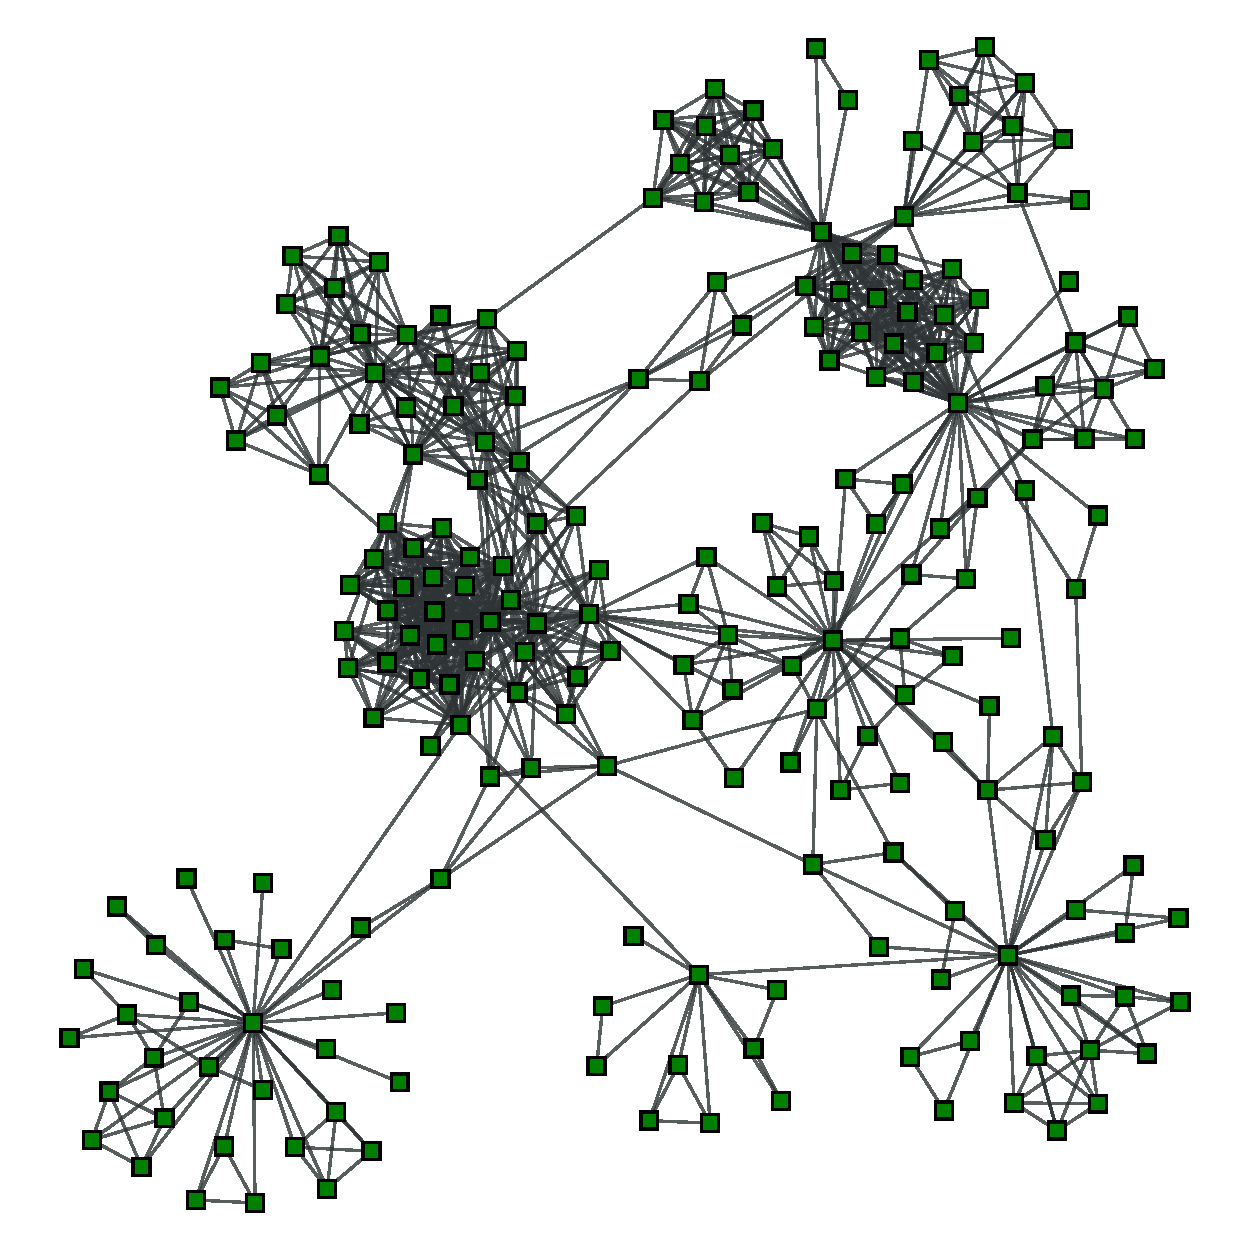
\includegraphics[width=0.8\columnwidth]{coauthors.pdf}
\end{frame}
%-------------------------
%-------------------------
\begin{frame}
    \frametitle{Community structure in networks}
    \centering
    {\bf What are communities?}
    \vspace{2em}
    \begin{itemize}
    \setlength\itemsep{1em}
        \item{{\bf Traditional definition}: Groups of nodes with a high internal link density}
        \item{{\bf Modern definition}: Nodes with similar connection probabilities to the rest of the network}
    \end{itemize}

\end{frame}
%-------------------------
%-------------------------
\begin{frame}
    \frametitle{Communities in the real-world networks}
    \centering
    \begin{itemize}
    \setlength\itemsep{1em}
        \item{{\bf Social networks}: 
            \begin{itemize}
                \item{Friend-circles}
                \item{Research communities}
                \item{Co-workers}
            \end{itemize}
    }
        \item{{\bf World Wide Web}: 
            \begin{itemize}
                \item{Pages with similar contents}
                \item{Webpages under the same domain (e.g. Wikipedia)}
            \end{itemize}
    }
        \item{{\bf Biological networks}:
            \begin{itemize}
                \item{Proteins with similar roles in protein interaction networks}
                \item{Chemicals together taking part in chemical reactions in metabolic networks}
                \item{Communities in neuronal networks}
            \end{itemize}
}
    \end{itemize}
\end{frame}
%-------------------------
%-------------------------
\begin{frame}
    \frametitle{Community detection}
    \centering
    
    {\bf Detecting communities is important!}
    \vspace{2em}
    \begin{itemize}
    \setlength\itemsep{1em}
        \item{Communities are building blocks of networks}
        \item{Communities allow us to see ``the big picture''}
        \item{Functional/Autonomous units}
        \item{Non-trivial effects on the processes on networks}
    \end{itemize}
\end{frame}
%-------------------------
%-------------------------
\begin{frame}
    \frametitle{Graph partitioning}
    \centering
    Problem of dividing a graph in a given number of groups of given sizes such that the number of links between the groups ({\bf cut size}) is minimized

    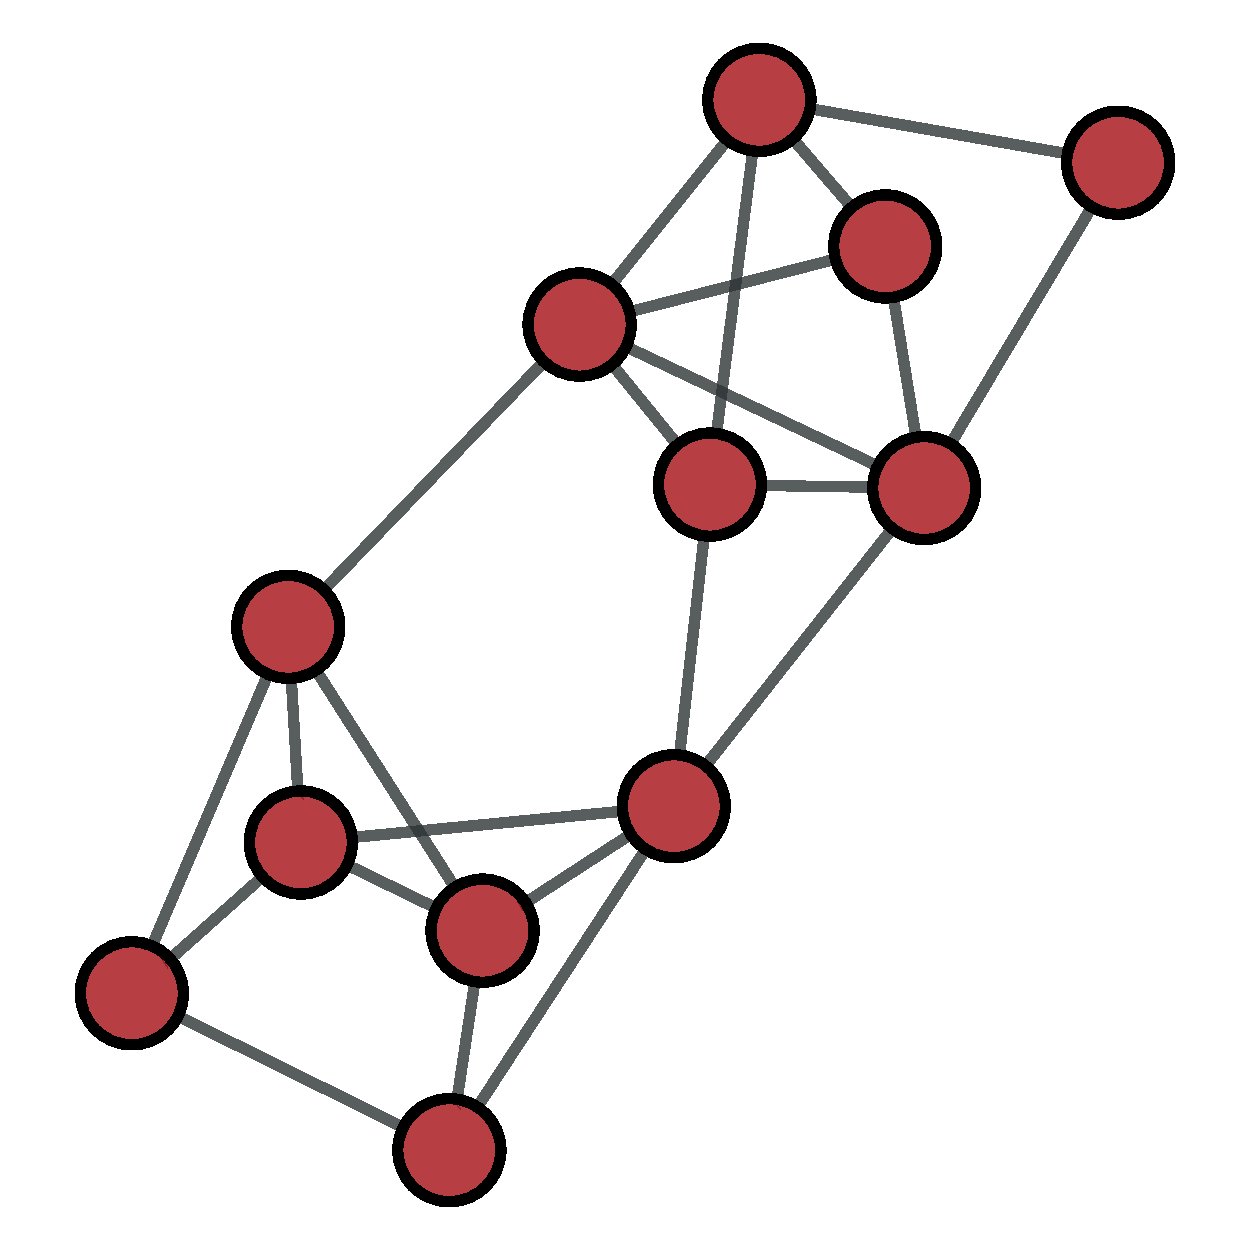
\includegraphics[width=0.5\columnwidth]{moderate_sized_network1.pdf}
\end{frame}
%-------------------------
%-------------------------
\begin{frame}
    \frametitle{Graph partitioning}
    \centering
    Problem of dividing a graph in a given number of groups of given sizes such that the number of links between the groups ({\bf cut size}) is minimized

    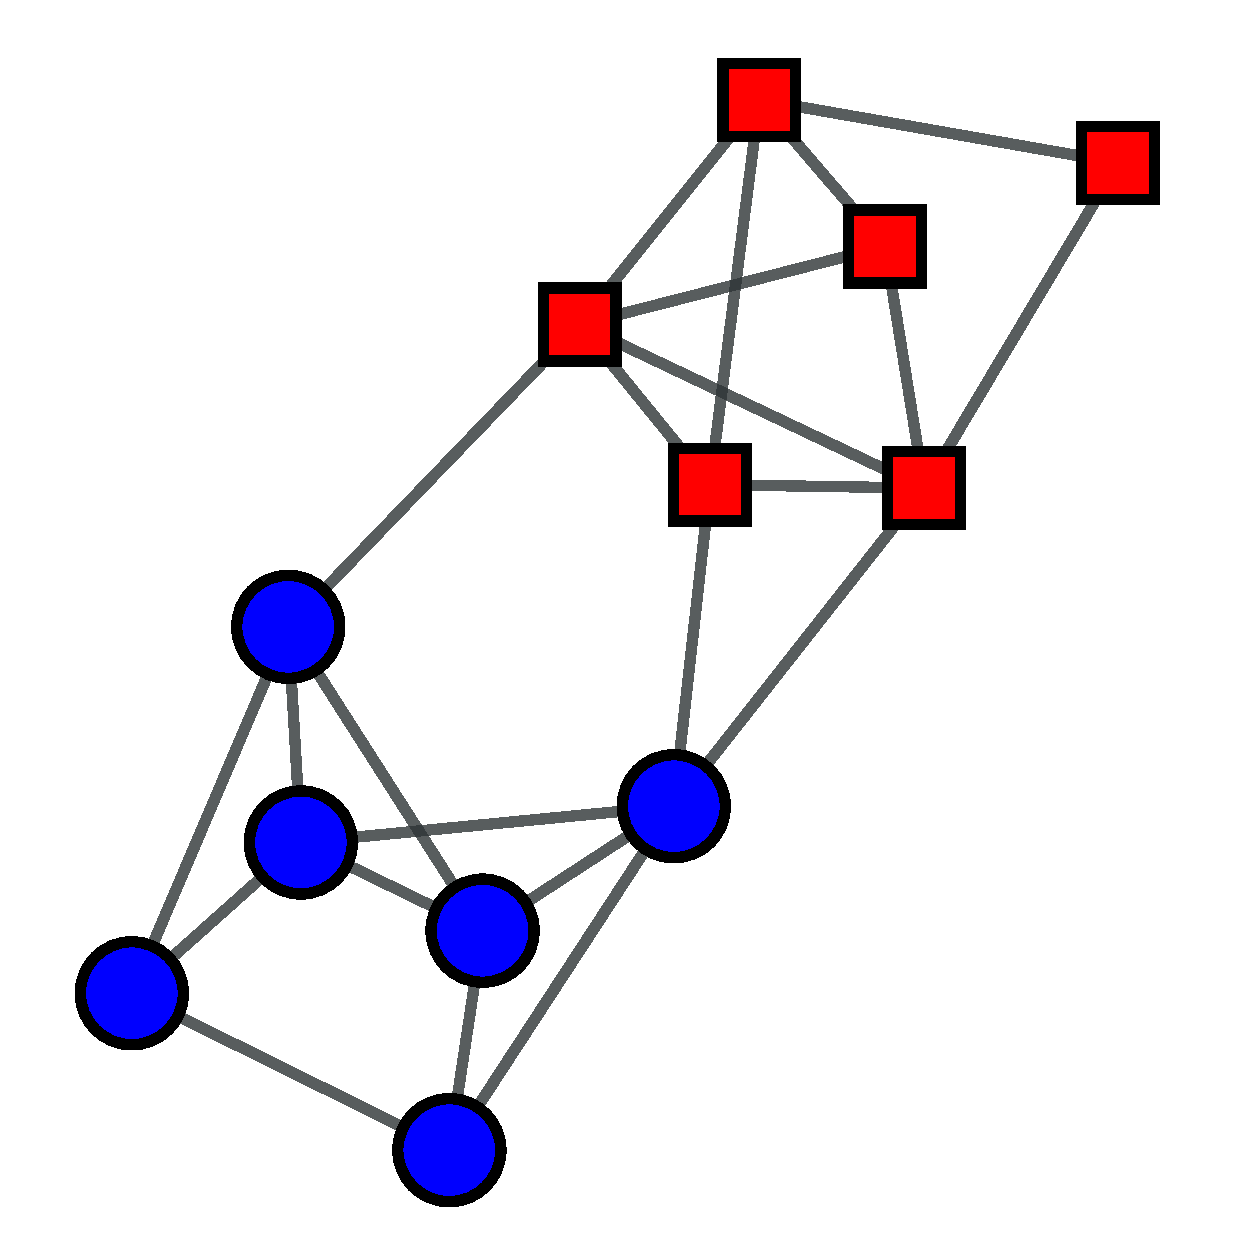
\includegraphics[width=0.5\columnwidth]{moderate_sized_network2.pdf}
\end{frame}
%-------------------------
%-------------------------
\begin{frame}
    \frametitle{Partitioning is hard!}
   \centering 
    \begin{itemize}
    \setlength\itemsep{1em}
        \item{Graph with $n$ vertices}
        \item{Find two groups with sizes $n_1$ and $n_2$ such that the cut size is minimum}
        \item{Number of ways: $\frac{n!}{n_1!n_2!}\approx \frac{2^{n+1}}{\sqrt{n}}$}
    \end{itemize}
    \vspace{20pt}
    {\bf Heuristics are needed!}
\end{frame}
%-------------------------
%-------------------------
\begin{frame}
    \frametitle{Kernighan-Lin algorithm}
    \begin{columns}
        \column{0.6\linewidth}
        \centering
        {\bf cut size = $4$}
        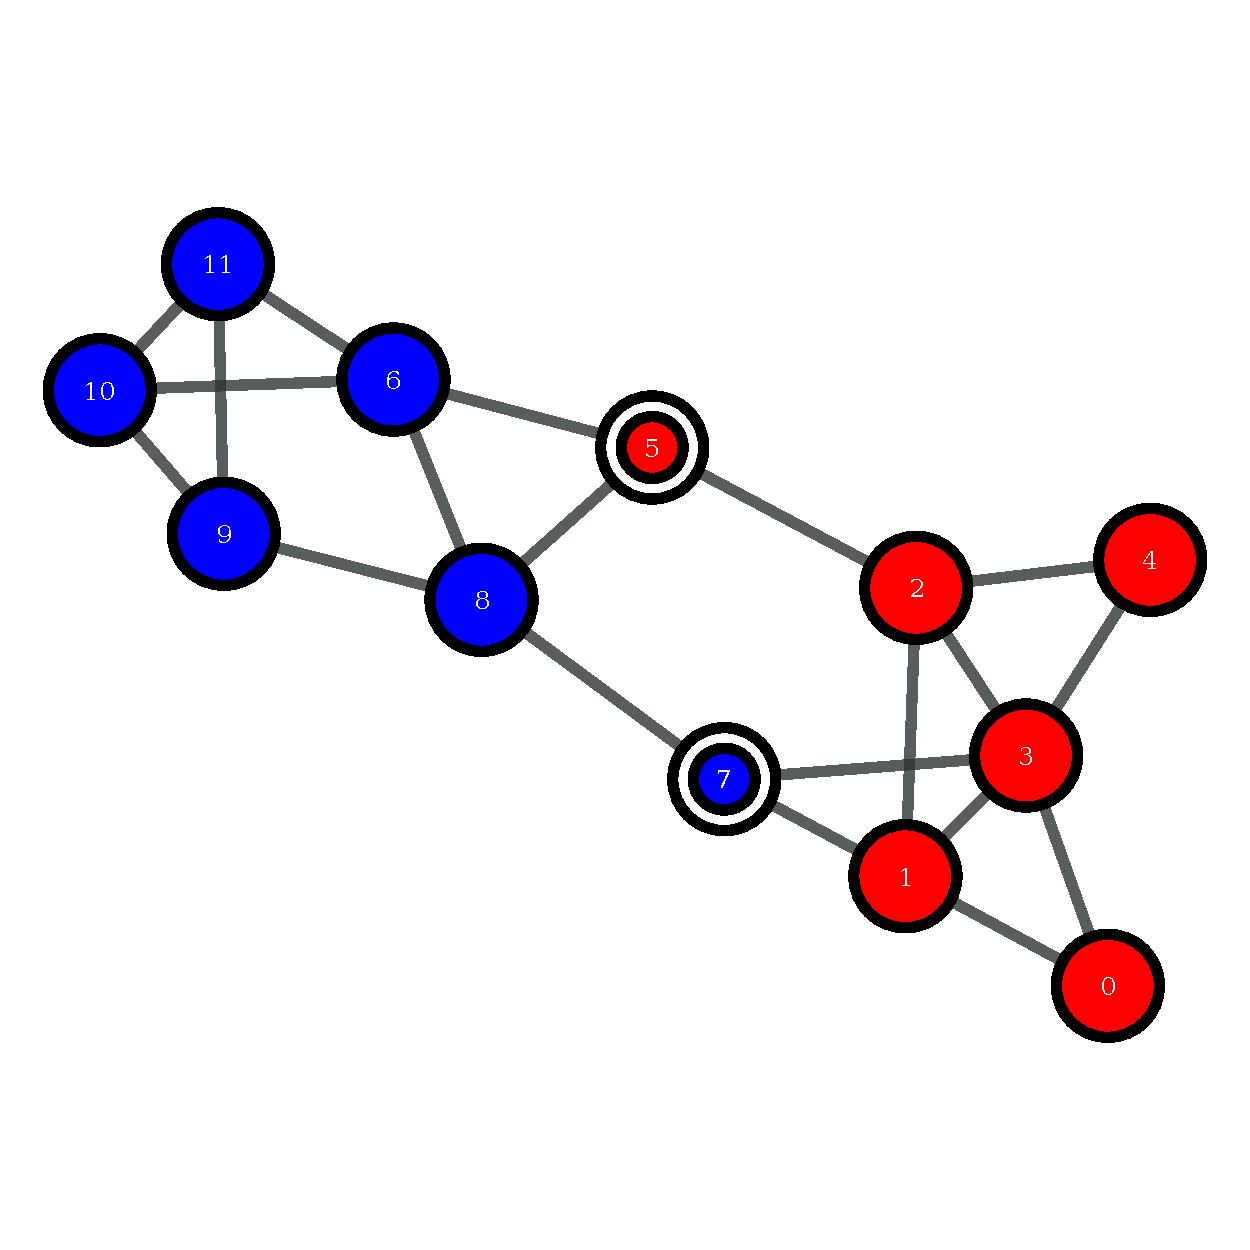
\includegraphics[width=0.8\columnwidth]{kl1.pdf}

        \column{0.5\linewidth}
        \centering
        \begin{itemize}
            \setlength\itemsep{1em}
            \item{\small Divide the vertices into two groups of the required sizes and calculate the cut size}
                \pause
            \item{\small Find a pair of nodes which when switched, will reduce the cut size most and switch them}
        \end{itemize}
    \end{columns}
\end{frame}
%-------------------------
%-------------------------
\begin{frame}
    \frametitle{Kernighan-Lin algorithm}
    \begin{columns}
        \column{0.6\linewidth}
        \centering
        {\bf cut size = $2$}
        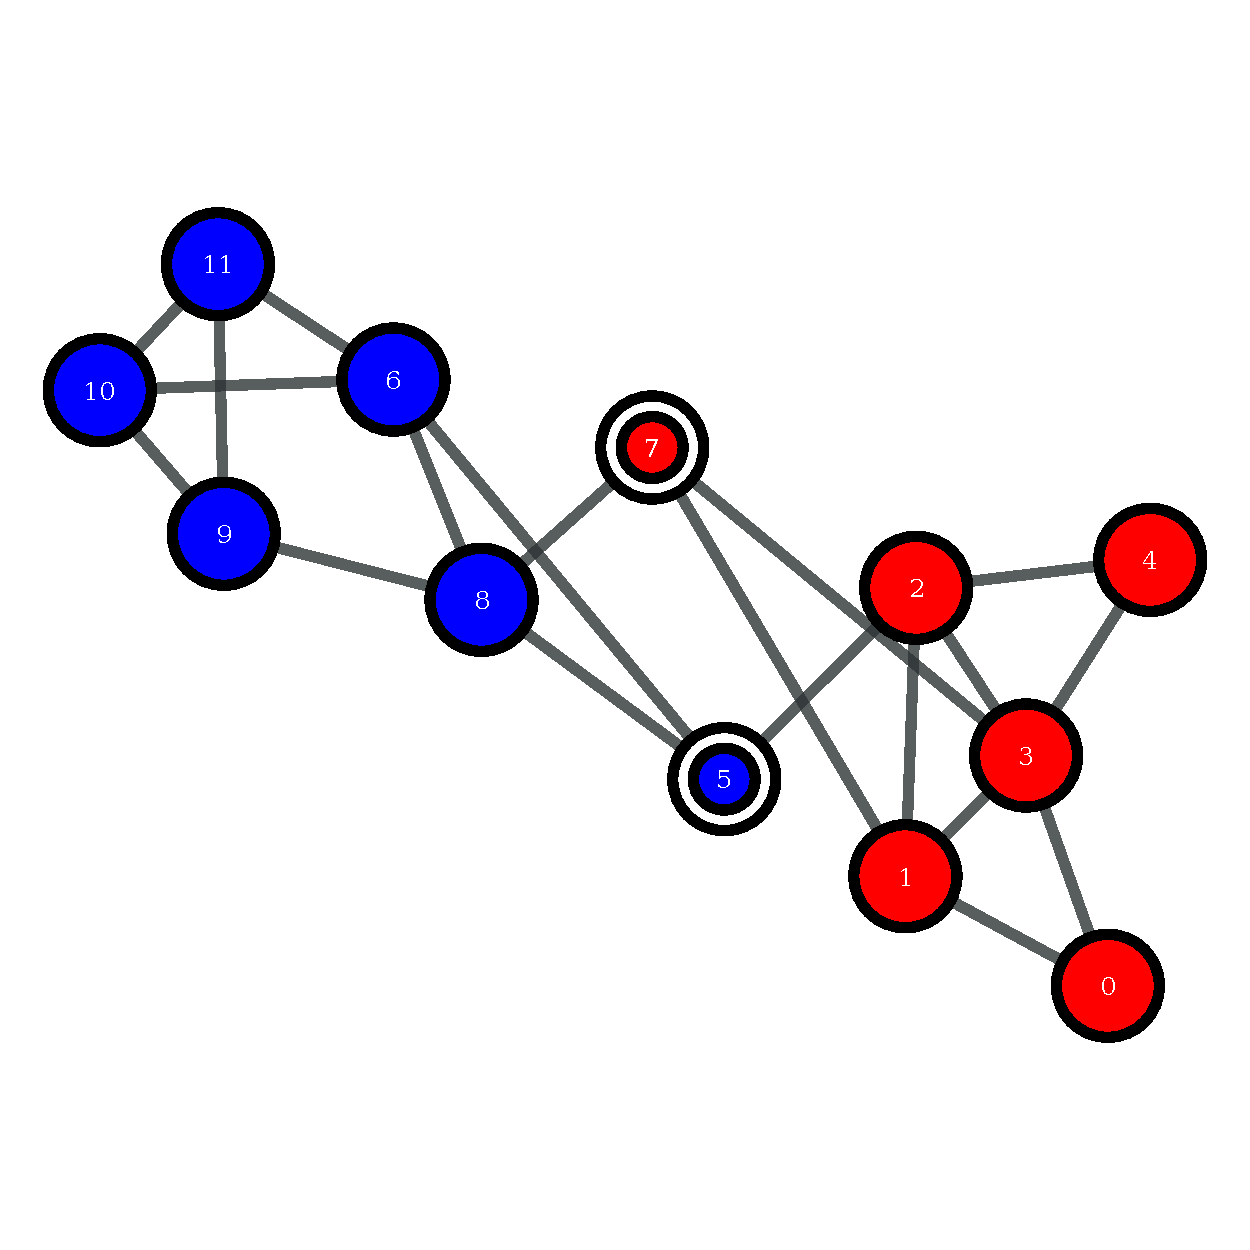
\includegraphics[width=0.8\columnwidth]{kl2.pdf}

        \column{0.5\linewidth}
        \centering
        \begin{itemize}
            \setlength\itemsep{1em}
            \item{\small Divide the vertices into two groups of the required sizes}
            \item{\small Find a pair of nodes which when switched, will reduce the cut size most and switch them}
                \pause
            \item{\small If no such pair exists, select the pair which least increases the cut size}
                \pause
            \item{\small Continue this such that the already switched pair is not switched again}
        \end{itemize}
    \end{columns}
\end{frame}
%-------------------------
%-------------------------
\begin{frame}
    \frametitle{Kernighan-Lin algorithm}
    \begin{itemize}
        \setlength\itemsep{1em}
        \item{Go through all the states and select the one with the least cut size}
        \item{Start with this state and repeat the whole procedure}
        \item{Continue till the cut size no longer becomes smaller}
            \note<1>{Group sizes remain constant}
        \item{Starting with many random initial conditions is better}
    \end{itemize}
\end{frame}
%-------------------------
%-------------------------
\begin{frame}
    \frametitle{Spectral partitioning}
    \centering

    \begin{itemize}
        \setlength\itemsep{1em}
        \item{Faster algorithm than Kernighan-Lin}
        \item{Uses properties of the graph Laplacian}
        \item{More complex to implement than Kernighan-Lin}
    \end{itemize}
\end{frame}
%-------------------------
%-------------------------
\begin{frame}
    \frametitle{Spectral partitioning}
Cut size:
$$R = \frac{1}{2}\sum\limits_{\substack{i, j \ \text{in} \\ \text{different} \\ \text{groups}}}A_{ij}$$

Define
$$s_i = \begin{cases}+1 &\quad\text{if vertex } i\ \text{belongs to group} \ 1 \\-1 &\quad\text{if vertex } i\ \text{belongs to group} \ 2\end{cases}$$

Then
$$\frac{1}{2}(1-s_is_j) = \begin{cases}1 &\quad \text{if} \ i\ \text{and} \ j\ \text{are in different groups,}\\0 &\quad \text{if} \ i\ \text{and} \ j\ \text{are in the same group}\end{cases}$$
\end{frame}
%-------------------------
%-------------------------
\begin{frame}
    \frametitle{Spectral partitioning}
    $$R = \frac{1}{4}\sum\limits_{ij}A_{ij}(1-s_is_j)$$

First term,
$$\sum\limits_{ij}A_{ij} = \sum\limits_ik_i = \sum\limits_ik_is_i^2=\sum\limits_{ij}k_i\delta_{ij}s_is_j$$

$$R = \frac{1}{4}\sum\limits_{ij}(k_i\delta_{ij}-A_{ij})s_is_j = \frac{1}{4}\sum\limits_{ij}L_{ij}s_is_j$$

$$R = \frac{1}{4}{\mathbf s}^T{\mathbf L}{\mathbf s}$$
\note{L is so imp that we have a name for it! Laplacian\\ .\\ s is a columnvector\\ . \\L: structure, s: division\\ . \\ find s that minimizes R\\.\\Problem is hard, s takes only integer values\\.}
\end{frame}
%-------------------------
%-------------------------
\begin{frame}
    \frametitle{Relaxation method}
\begin{columns}
    \column{0.6\linewidth}
    \centering
%$$R = \frac{1}{4}{\bf s}^T{\bf L}{\bf s}$$
%\vspace{0.5em}

{\bf Two constraints}:
\vspace{1em}
    \begin{itemize}
    \setlength\itemsep{1em}
        %\item{$s_i$ can be only $\pm 1$ $\Rightarrow$ Length of ${\bf s}$ is $\sqrt{n}$}
        \item{$s_i$ can be only $\pm 1$}
        \item{$\sum\limits_{i}s_i=n_1-n_2 \Rightarrow {\mathbf 1}^T{\mathbf s} = n_1-n_2$}
    \end{itemize}

\centering
\vspace{2em}
Relax the first constraint
\column{0.4\linewidth}
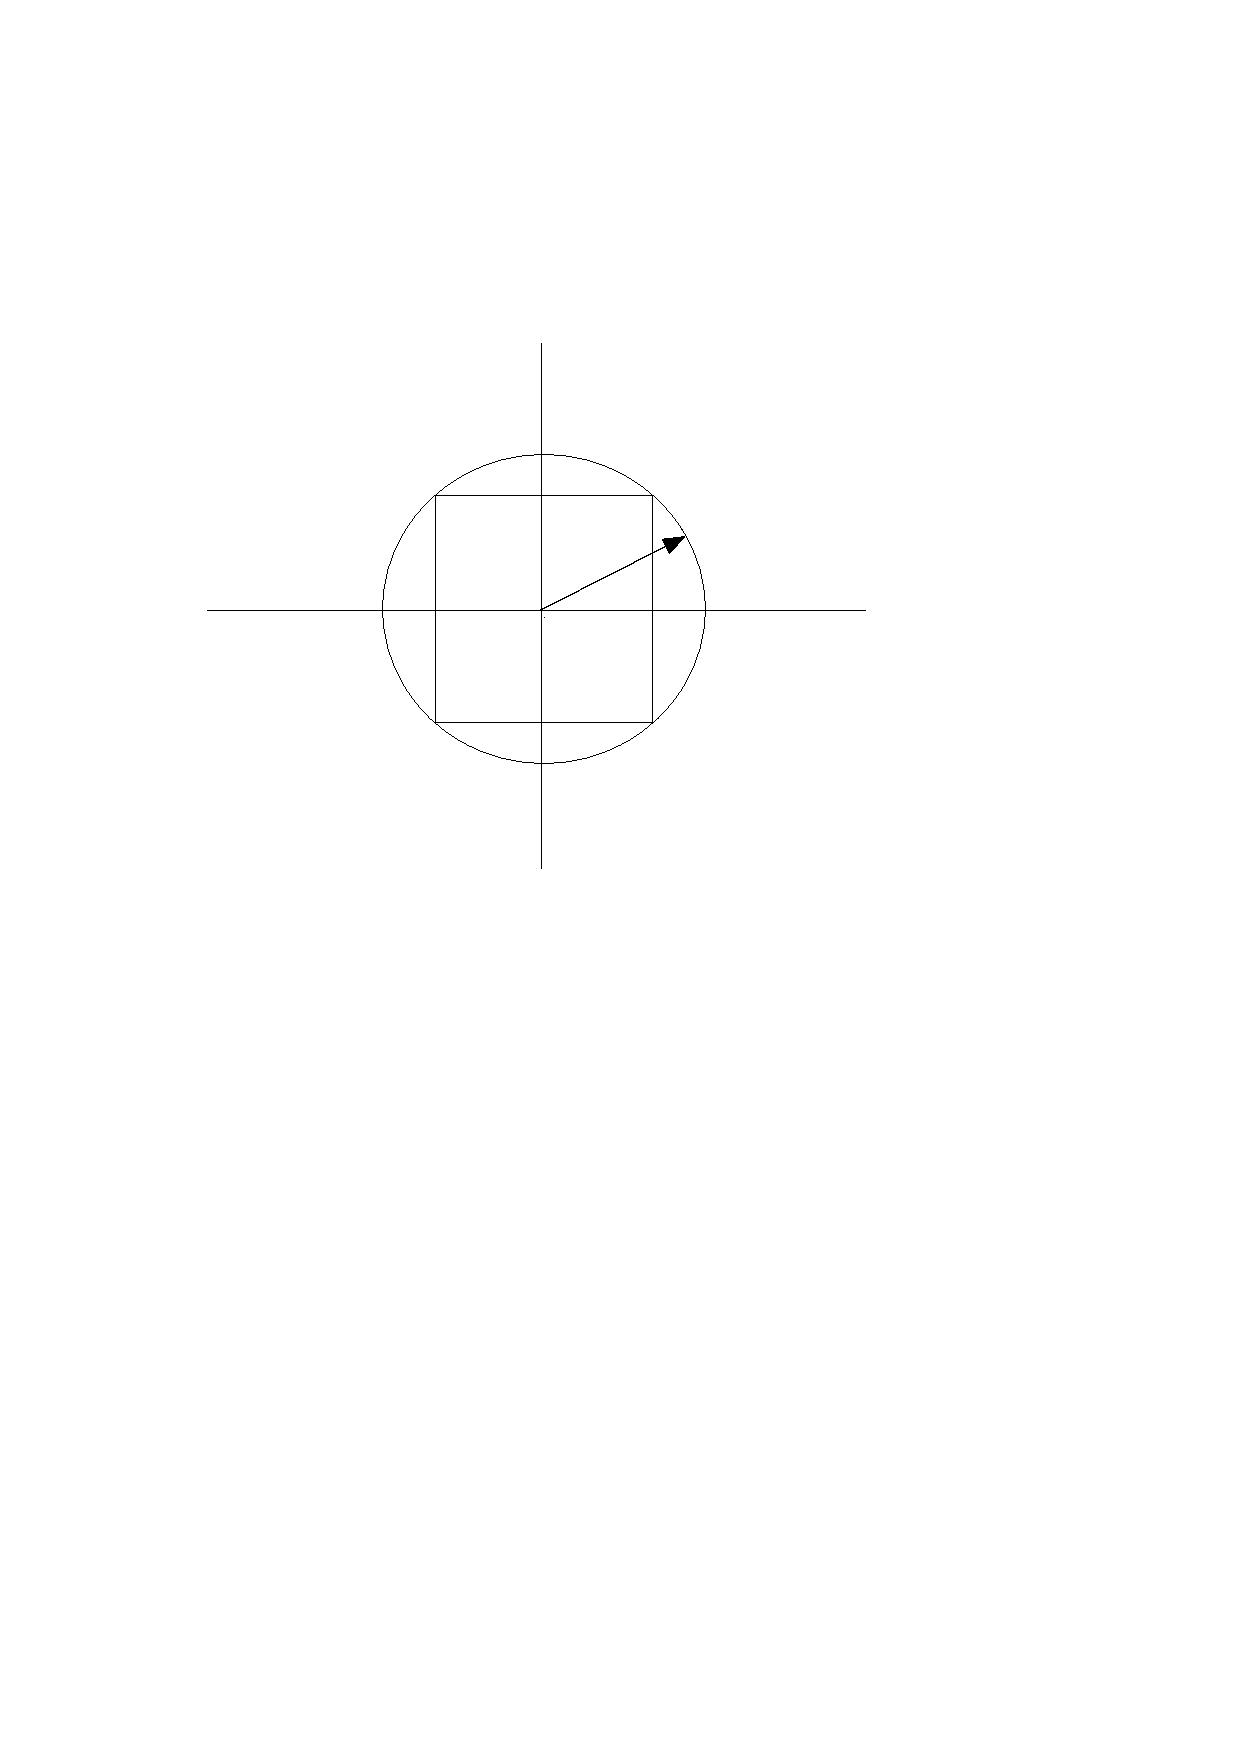
\includegraphics[width=\columnwidth,trim=100 400 200 200, clip=true]{hypercube.pdf}
\end{columns}
    \note{hypercube\\.\\continuous s, differentiate}
\end{frame}
%-------------------------
%-------------------------
\begin{frame}
    \frametitle{Spectral partitioning}
    \centering
Minimization with constraints $\Rightarrow$ Lagrange multipliers
    $$\frac{\partial}{\partial s_i}\left[\sum\limits_{jk}L_{jk}s_js_k + \lambda\left(n-\sum\limits_{j}s_j^2\right) + 2\mu\left((n_1-n_2)-\sum\limits_js_j\right)\right] = 0$$
    \pause
    $$\sum\limits_jL_{ij}s_j = \lambda s_i + \mu$$
\justifying
%In matrix notation,
    \pause
$${\mathbf L}{\mathbf s} = \lambda {\mathbf s} + \mu {\mathbf 1} = \lambda \left({\mathbf s} + \frac{\mu}{\lambda}{\mathbf 1}\right)$$
$${\mathbf L}\left({\mathbf s} + \frac{\mu}{\lambda}\right) = \lambda \left({\mathbf s} + \frac{\mu}{\lambda}{\mathbf 1}\right)$$
\end{frame}
%-------------------------
%-------------------------
\begin{frame}
    \frametitle{Community detection is harder!}
  \begin{itemize}
        \setlength\itemsep{2em}
        \item{{\bf Graph partitioning}
        \begin{itemize}
        \setlength\itemsep{0.5em}
            \item{\small well defined}
            \item{\small Number of groups is fixed}
            \item{\small Sizes of the groups are fixed}
            \item{\small Divide even if no good division exists}
        \end{itemize}
        }
        \item{{\bf Community detection}
        \begin{itemize}
        \setlength\itemsep{0.5em}
            \item{ill-defined}
            \item{\small Number of groups depends on the structure of the network}
            \item{\small Sizes of the groups depend on the structure of the network}
            \item{\small Discover natural fault lines}
        \end{itemize}
        }
    \end{itemize}
\end{frame}
%-------------------------
%-------------------------
\begin{frame}
    \frametitle{Many definitions.. many algorithms!}
    \centering
    \begin{itemize}
    \setlength\itemsep{1em}
            \note<1>{I can go on.. These algorithms use different definitions/views of communities}
        \item{Girvan-Newman algorithm}
        \item{Kernighan-Lin-Newman algorithm}
        \item{Spectral decomposition}
        \item{Clique-percolation}
        \item{Radom walk methods}
        \item{Statistical inference}
        \item{Label propagation}
        \item{Hierarchical clustering}
    \end{itemize}
\end{frame}
%-------------------------
%-------------------------
\begin{frame}
    \frametitle{Broad classification}
    \centering
    \begin{itemize}
        \setlength\itemsep{0.5em}
        \item{{\bf Agglomerative algorithms:}
            
    \begin{itemize}
        \setlength\itemsep{0.5em}
        \item{Hierarchical clustering}
        \item{Louvain method}
        \item{CNM algorithm}
    \end{itemize}
            
            }
        \item{{\bf Divisive algorithms:}
            
    \begin{itemize}
        \setlength\itemsep{0.5em}
        \item{\textcolor{brown}{Girvan-Newman algorithm}}
        \item{Radichhi algorithm}
    \end{itemize}
            
            
            }
        \item{{\bf Assignment algorithms:}

    \begin{itemize}
        \setlength\itemsep{1em}
        \item{Label propagation}
        \item{\textcolor{brown}{Spectral partitioning}}
        \item{\textcolor{brown}{Kernighan-Lin-Newman algorithm}}
    \end{itemize}

            }
    \end{itemize}
\end{frame}
%-------------------------
%-------------------------
\begin{frame}
    \frametitle{``The'' simplest community detection problem}
    \centering
    \begin{itemize}
    \setlength\itemsep{1em}
        \item{Bisecting a graph with $n$ nodes}
        \item{Group sizes are not fixed}
        \item{Minimum cut size?}
            \note<1>{Empty group}
    \end{itemize}
    \note<2>{Different measure}

    \vspace{2em}
    \pause
    {\bf A different measure of the quality of division is required..}
\end{frame}
%-------------------------
%-------------------------
\begin{frame}
    \frametitle{Quantification of community structure}
    \centering

    \begin{itemize}
        \setlength\itemsep{1em}
        \item{Fewer than expected edges between the groups}
            \note<1>{few edges = expected edges = not a good division}
            \note<2>{Remember assortativity}
            \pause
        \item{Equivalently, more than expected edges inside the groups}
            \pause
            \note<3>{Divide network using modularity}
        \item{Assortativity mixing and modularity}
            \pause
        \item{Look for divisions with high modularity}
            \note<4>{Heuristics are needed}
            \pause
        \item{Modularity maximization is hard}
    \end{itemize}

\end{frame}
%-------------------------
%-------------------------
\begin{frame}
    \frametitle{Newman-Girvan algorithm}
    \centering
    
    \begin{itemize}
        \setlength\itemsep{1em}
        \item{Look for edges between the communities}

            %\note<1>{Number of shortest paths that pass through a given edge}
            \note<1>{Let's have a look at the edge betweenness}
        \item{Edge betweenness}
    \end{itemize}
\end{frame}
%-------------------------
%-------------------------
\begin{frame}
    \frametitle{Edge betweenness}
    \centering
    \vspace{2em}
        \begin{itemize}
        \setlength\itemsep{1em}
            \item{Path between two nodes}
            \item{Shortest path between two nodes}
            \item{Number of shortest paths that go through a given edge}
        \end{itemize}
    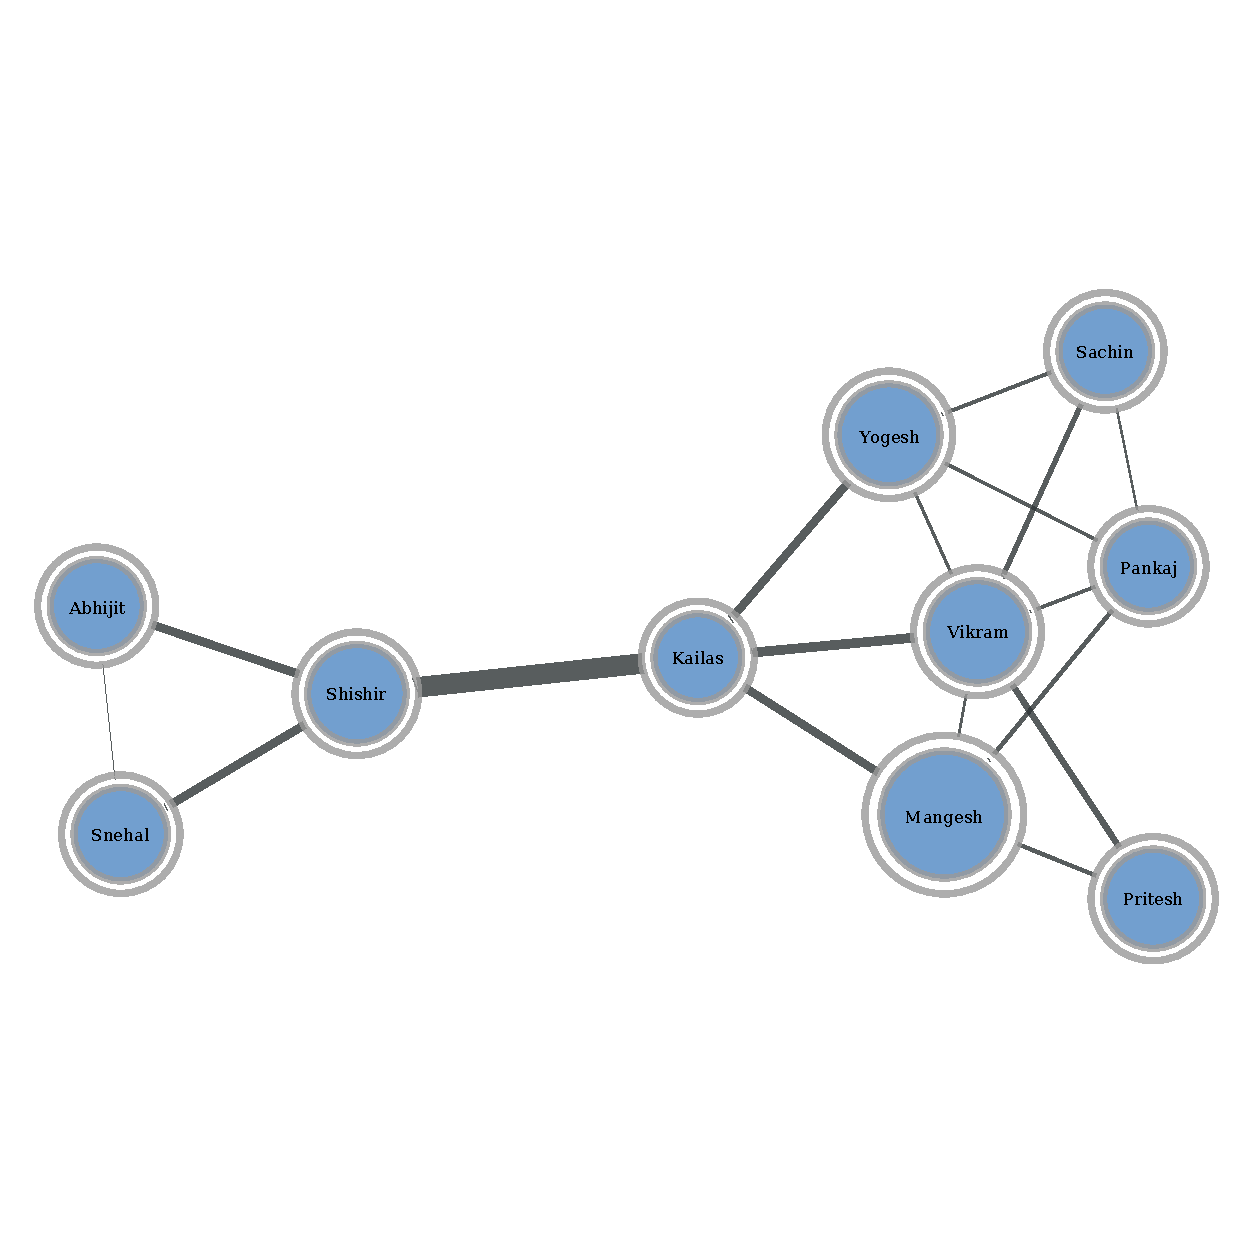
\includegraphics[width=0.7\columnwidth,trim=0 0 0 130,clip=true]{msc3.pdf}

\end{frame}
%-------------------------
%-------------------------
\begin{frame}
    \frametitle{The algorithm}
    \centering

    \begin{itemize}
    \setlength\itemsep{1em}
        \item{Calculate betweenness for all edges}
        \item{Remove the edge with the highest betweenness}
        \item{Recalculate betweenness for all edges}
        \item{Repeat}
    \end{itemize}
\end{frame}
%-------------------------
%%-------------------------
%\begin{frame}
%    \frametitle{}
%    \centering
%\end{frame}
%%-------------------------
%%-------------------------
%\begin{frame}
%    \frametitle{}
%    \centering
%\end{frame}
%%-------------------------
%%-------------------------
%\begin{frame}
%    \frametitle{}
%    \centering
%\end{frame}
%%-------------------------
%%-------------------------
%\begin{frame}
%    \frametitle{}
%    \centering
%\end{frame}
%%-------------------------
%%-------------------------
%\begin{frame}
%    \frametitle{}
%    \centering
%\end{frame}
%%-------------------------
%%-------------------------
%\begin{frame}
%    \frametitle{}
%    \centering
%\end{frame}
%%-------------------------
%%-------------------------
%\begin{frame}
%    \frametitle{}
%    \centering
%\end{frame}
%%-------------------------
%%-------------------------
%\begin{frame}
%    \frametitle{}
%    \centering
%\end{frame}
%%-------------------------
%%-------------------------
%\begin{frame}
%    \frametitle{}
%    \centering
%\end{frame}
%%-------------------------
%%-------------------------
%\begin{frame}
%    \frametitle{}
%    \centering
%\end{frame}
%%-------------------------
%%-------------------------
%\begin{frame}
%    \frametitle{}
%    \centering
%\end{frame}
%%-------------------------
%%-------------------------
%\begin{frame}
%    \frametitle{}
%    \centering
%\end{frame}
%%-------------------------
%%-------------------------
%\begin{frame}
%    \frametitle{}
%    \centering
%\end{frame}
%%-------------------------
%%-------------------------
%\begin{frame}
%    \frametitle{}
%    \centering
%\end{frame}
%%-------------------------
%%-------------------------
%\begin{frame}
%    \frametitle{}
%    \centering
%\end{frame}
%%-------------------------
%%-------------------------
%\begin{frame}
%    \frametitle{}
%    \centering
%\end{frame}
%%-------------------------
%%-------------------------
%\begin{frame}
%    \frametitle{}
%    \centering
%\end{frame}
%%-------------------------
%%-------------------------
%\begin{frame}
%    \frametitle{}
%    \centering
%\end{frame}
%%-------------------------
%%-------------------------
%\begin{frame}
%    \frametitle{}
%    \centering
%\end{frame}
%%-------------------------
%%-------------------------
%\begin{frame}
%    \frametitle{}
%    \centering
%\end{frame}
%%-------------------------
%%-------------------------
%\begin{frame}
%    \frametitle{}
%    \centering
%\end{frame}
%%-------------------------
%%-------------------------
%\begin{frame}
%    \frametitle{}
%    \centering
%\end{frame}
%%-------------------------
%%-------------------------
%\begin{frame}
%    \frametitle{}
%    \centering
%\end{frame}
%%-------------------------
%%-------------------------
%\begin{frame}
%    \frametitle{}
%    \centering
%\end{frame}
%%-------------------------
%%-------------------------
%\begin{frame}
%    \frametitle{}
%    \centering
%\end{frame}
%%-------------------------
%%-------------------------
%\begin{frame}
%    \frametitle{}
%    \centering
%\end{frame}
%%-------------------------
%%-------------------------
%\begin{frame}
%    \frametitle{}
%    \centering
%\end{frame}
%%-------------------------
%%-------------------------
%\begin{frame}
%    \frametitle{}
%    \centering
%\end{frame}
%%-------------------------
%%-------------------------
%\begin{frame}
%    \frametitle{}
%    \centering
%\end{frame}
%%-------------------------
\end{document}
